% Created 2017-04-13 Thu 16:17
% Intended LaTeX compiler: pdflatex
\documentclass[a4paper,11pt]{article}
\usepackage[utf8]{inputenc}
\usepackage[T1]{fontenc}
\usepackage{graphicx}
\usepackage{grffile}
\usepackage{longtable}
\usepackage{wrapfig}
\usepackage{rotating}
\usepackage[normalem]{ulem}
\usepackage{amsmath}
\usepackage{textcomp}
\usepackage{amssymb}
\usepackage{capt-of}
\usepackage{hyperref}
\usepackage[margin=1in]{geometry}
\usepackage{setspace}
\onehalfspacing
\usepackage{parskip}
\usepackage{mathtools}
\usepackage{hyperref}
\hypersetup{colorlinks,citecolor=black,filecolor=black,linkcolor=black,urlcolor=black}
\usepackage{graphicx}
\usepackage{tabularx}
\usepackage{color}
\usepackage[font={footnotesize}]{caption}
\newtheorem{mydef}{Definition}
\newtheorem{mythm}{Theorem}
\newcommand{\dx}{\mathrm{d}}
\newcommand{\var}{\mathrm{Var}}
\newcommand{\cov}{\mathrm{Cov}}
\newcommand{\corr}{\mathrm{Corr}}
\newcommand{\pr}{\mathrm{Pr}}
\newcommand{\rarrowd}[1]{\xrightarrow{\text{ \textit #1 }}}
\DeclareMathOperator*{\plim}{plim}
\newcommand{\plimn}{\plim_{n \rightarrow \infty}}
\setcounter{secnumdepth}{2}
\author{Zheng Tian}
\date{}
\title{Lecture 2: The ARCH Model}
\hypersetup{
 pdfauthor={Zheng Tian},
 pdftitle={Lecture 2: The ARCH Model},
 pdfkeywords={},
 pdfsubject={},
 pdfcreator={Emacs 25.1.1 (Org mode 9.0.3)}, 
 pdflang={English}}
\begin{document}

\maketitle

\section{The Volatility of Asset Returns}
\label{sec:org1c2263d}

This lecture focuses on the volatility of asset returns. Here
volatility refers to the \textbf{conditional variance} of a time series. That
is, for a return series \{\(r_t\)\}, we are now interested in 
\[\sigma^2_t = \var(r_t \mid F_{t-1})\]
where \(F_{t-1}\) is the information set at time \(t-1\). 

\subsection{Characteristics of volatility}
\label{sec:orgf33d1dd}

In practice, we have observed some stylized facts about volatility,
and some volatility models are proposed to characterize them. These
properties of volatility include:

\begin{enumerate}
\item There exist volatility clusters. That is, volatility may be high
for certain time periods and low for other periods. Figure
\ref{fig:org9ac2999} shows the daily changes in the log of the NYSE
U.S. 100 stock price index. As seen, a cluster of tranquil periods
from 2003 to 2007 is followed by a cluster of drastic volatile
periods from 2008 to 2010. 

\begin{figure}[htbp]
\centering
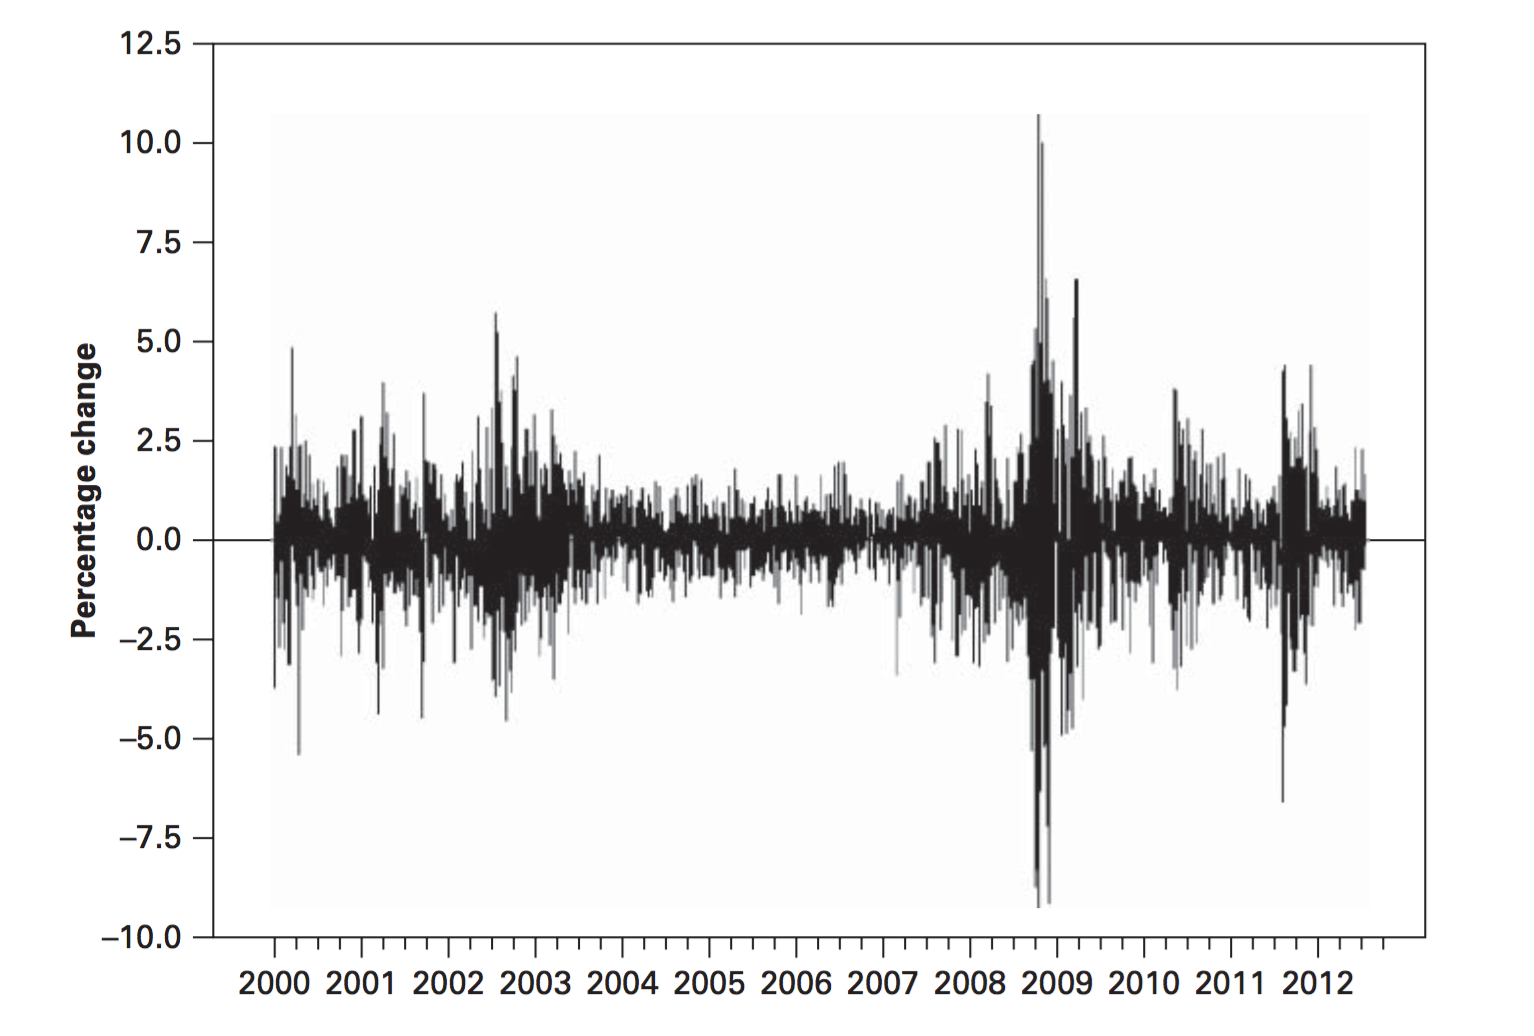
\includegraphics[width=\textwidth]{img/nyse_us100.png}
\caption{\label{fig:org9ac2999}
Percentage Change in the NYSE U.S. 100}
\end{figure}

\item Volatility evolves over time in a continuous manner. That is,
volatility jumps are rare. In Figure \ref{fig:org9ed4c08}, the change of the
volatility of the annualized real GDP growth rate of the U.S. is
relatively smooth. 

\begin{figure}[htbp]
\centering
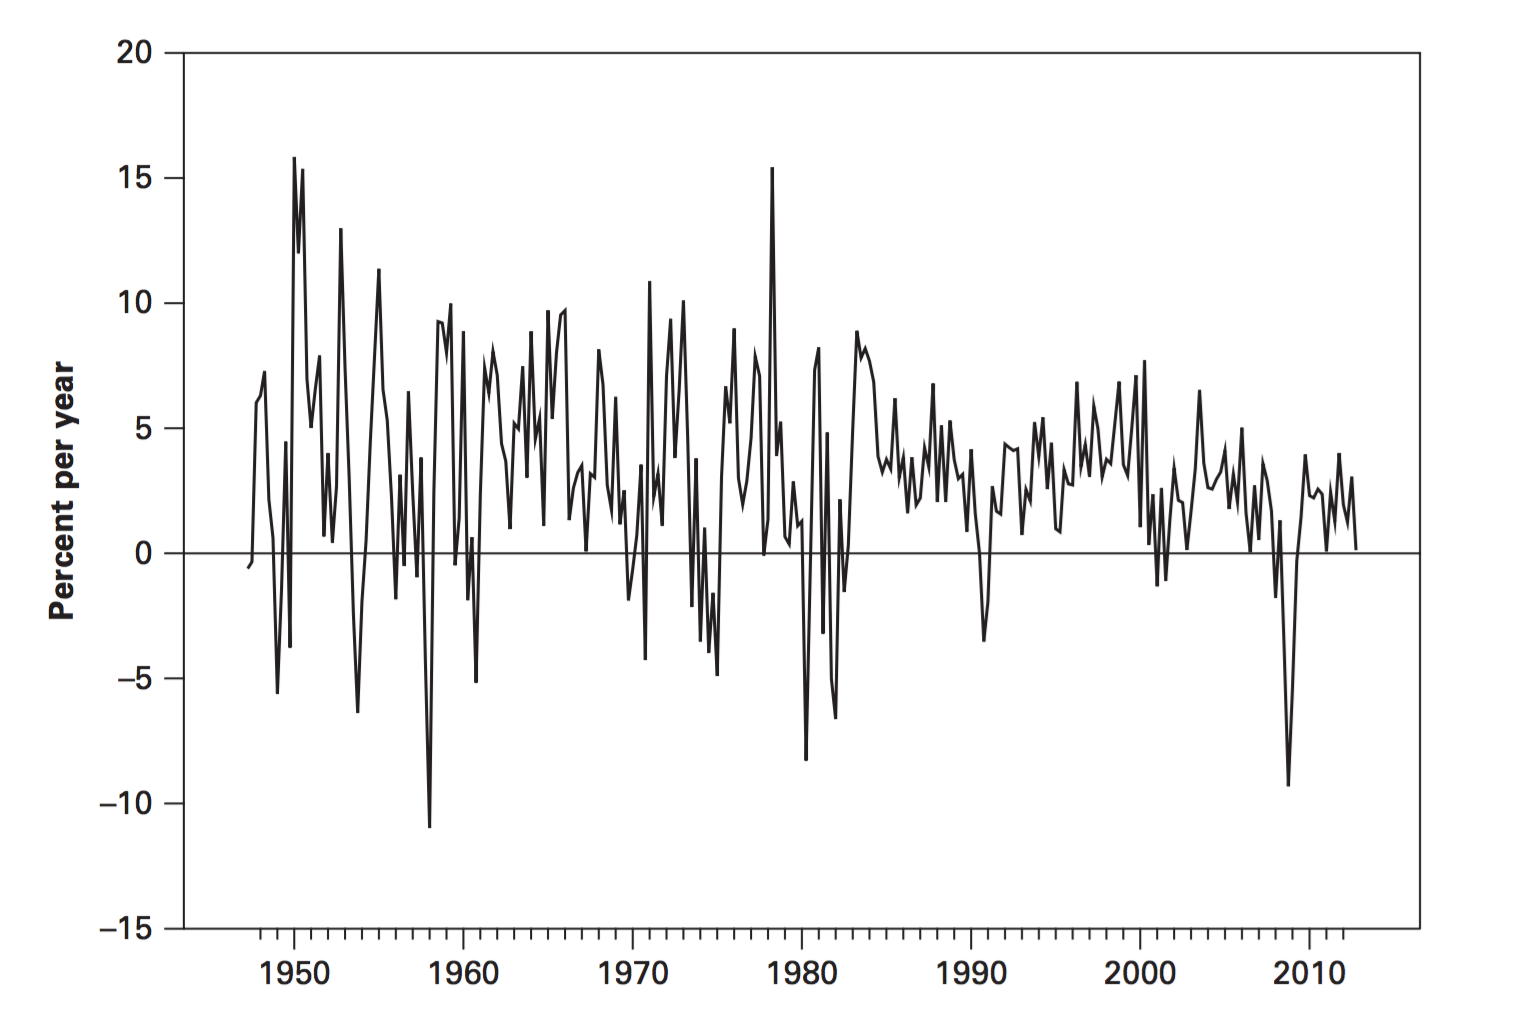
\includegraphics[width=\textwidth]{img/readgdp.png}
\caption{\label{fig:org9ed4c08}
Annualized Growth Rate of Real GDP}
\end{figure}

\item Volatility does not diverge to infinity. That is, volatility varies
within some fixed range. Statistically speaking, this means that
volatility is often stationary.

\item Volatility seems to react differently to a big price increase or a
big price drop, referred to as the leverage effect.
\end{enumerate}


\section{The Structure of a Volatility Model}
\label{sec:orgd1118c3}

\subsection{The basic idea of building a volatility model}
\label{sec:org5c37adf}
Consider the log return series \{\(r_t\)\}. The basic idea of a volatility
model is that \{\(r_t\)\} may appear to be either serially uncorrelated or
serially correlated with a minor order, but \{\(r_t\)\} is a dependent
series and the dependence arises from its conditional variance. 

\begin{figure}[htbp]
\centering
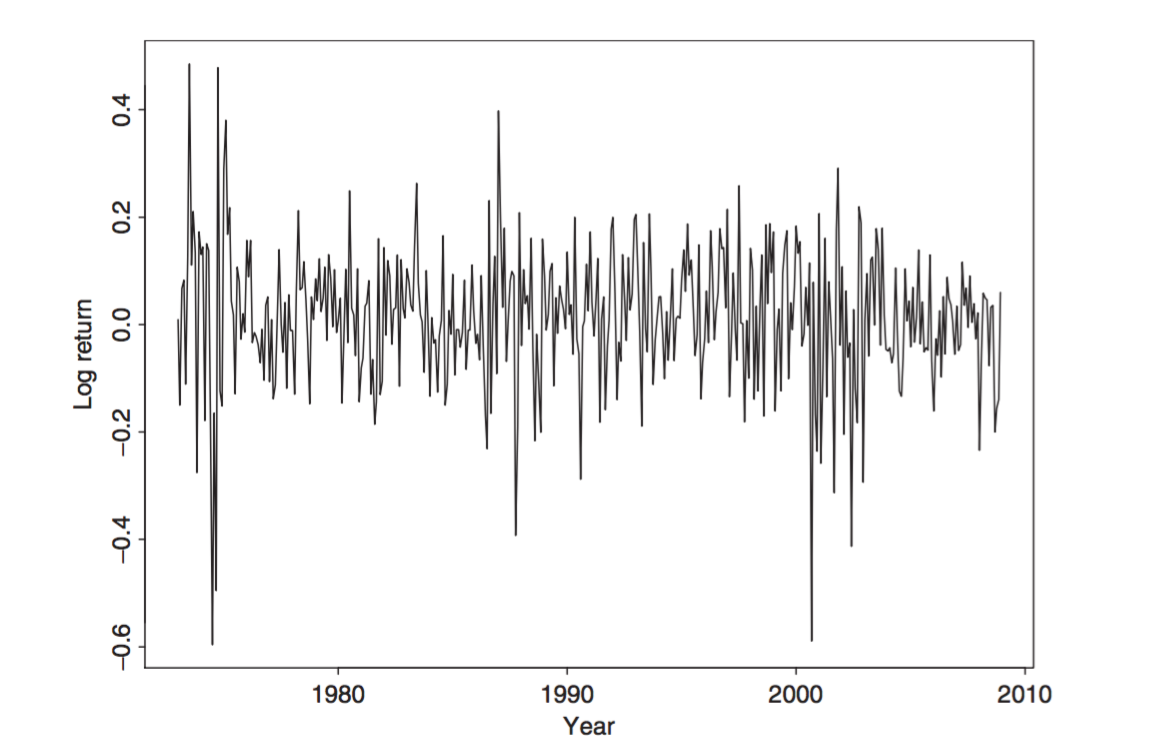
\includegraphics[width=\textwidth]{img/intel.png}
\caption{\label{fig:orgd514d82}
Time plot of monthly log returns of Intel stock from January 1973 to December 2008}
\end{figure}

\begin{figure}[htbp]
\centering
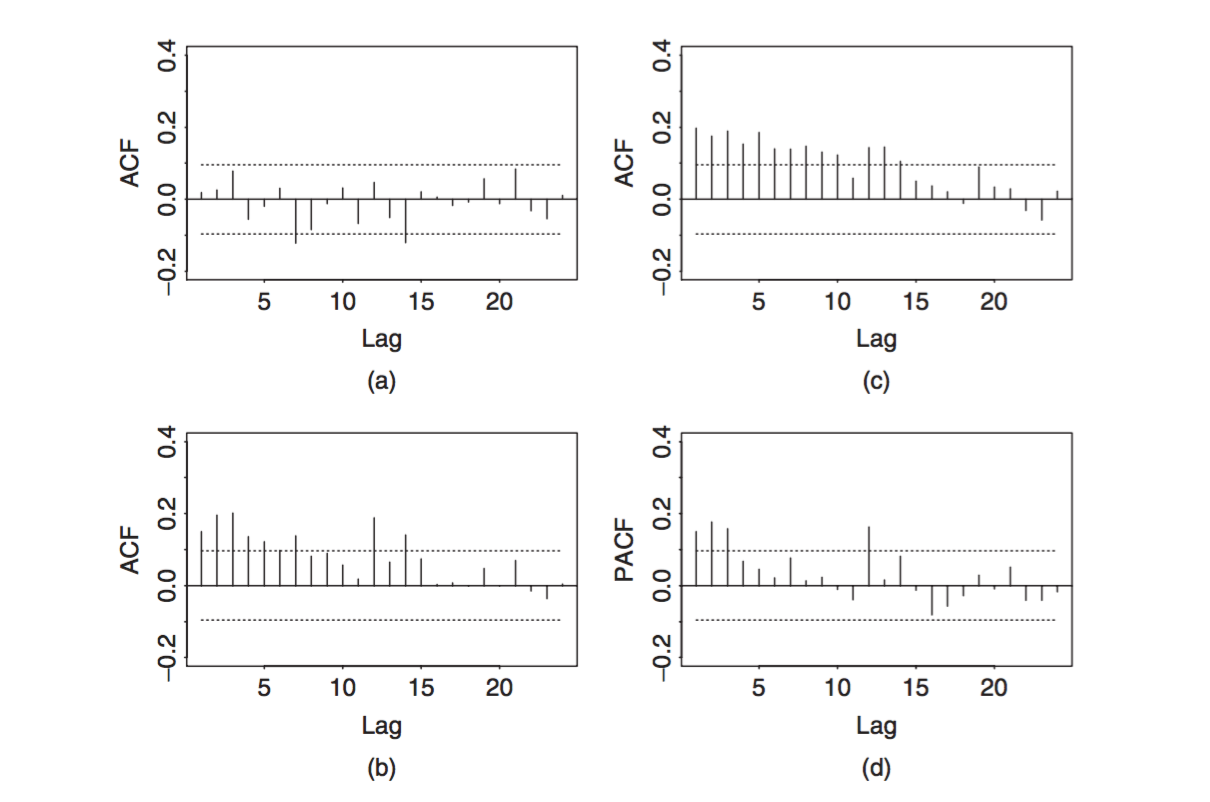
\includegraphics[width=\textwidth]{img/acf_intel.png}
\caption{\label{fig:orga23ad1d}
Sample ACF and PACF of various functions of monthly log stock returns of Intel Corporation from January 1973 to December 2008: (a) ACF of the log returns, (b) ACF of the squared log returns, (c) ACF of the absolute log returns, and (d) PACF of the squared log returns.}
\end{figure}

For illustration, consider the monthly log stock returns of Intel
Corporation from January 1973 to December 2008 shown in Figure
\ref{fig:orgd514d82}. 

Figure \ref{fig:orga23ad1d} displays the sample ACF and PACF of the
log return. 
\begin{itemize}
\item Figure \ref{fig:orga23ad1d}(a) shows the sample ACF of the log
return series \{\(r_t\)\}, which suggests no significant serial correlations
except for a minor one at lag 7.
\item Figure \ref{fig:orga23ad1d}(b) shows the sample ACF of the squared log returns
\{\(r^2_t\)\}.
\item Figure  \ref{fig:orga23ad1d}(c) shows the sample ACF of the absolute log returns,
\end{itemize}

These two plots clearly suggest that the monthly log returns are not
serially independent. Combining the three plots, it seems that the
log returns are indeed serially uncorrelated but
dependent. Volatility models attempt to capture such dependence in
the return series.

\subsection{The mean equation and the volatility equation}
\label{sec:org0538c97}

\subsection{The procedure of building a volatility model}
\label{sec:orgb68b0ad}

\subsection{Testing for the presence of ARCH effect}
\label{sec:org2b05250}


\section{The ARCH Model}
\label{sec:orgee0d333}

\subsection{The ARCH(m) Model}
\label{sec:orgb4fe980}

\subsection{The properties of ARCH models}
\label{sec:org4772dd5}

\subsection{Order determination}
\label{sec:orgd985543}

\subsection{Estimation}
\label{sec:org06c71d0}

\subsection{Model checking}
\label{sec:orga281be8}


\section{Applications with R}
\label{sec:orga19da55}
\end{document}